\documentclass{article}
\usepackage[utf8]{inputenc}
\usepackage{graphicx}
\graphicspath{{images/}{../images/}}

\title{Secure Programming Summary}
\author{Jacob Burley}
\date{Block 2 2018}

\begin{document}

\maketitle

\tableofcontents
\newpage
\section{Introduction}
\subsection{What is security?}
The state of being secure
\\CIA: \textbf{only} authorised actors can:
\begin{itemize}
    \item Learn secrets (\textbf{Confidentiality})
    \begin{itemize}
        \item \textbf{Data Confidentiality}: make sure that private information is not available to unauthorised actors
        \item \textbf{Privacy}: Individuals have control over what information is collected and stored, and how that information is shared
    \end{itemize}
    \item Modify messages/data (\textbf{Integrity})
    \begin{itemize}
        \item \textbf{Data Integrity}: Assures that information is modified only in a way that is known
        \item \textbf{System Integrity}: Ensures that a system performs as designed, without unauthorised modification
    \end{itemize}
    \item Access messages/data (\textbf{Availability})
    \begin{itemize}
        \item \textbf{Availability}: ensures that service is provided to an acceptable level, without denying access to authorised users
    \end{itemize}
\end{itemize}
Security is best \textbf{by design} - not as afterthought
\subsection{Identifying requirements for a secure protocol}
\begin{itemize}
    \item Always work towards CIA protocols described above
    \item We can do this by using the following three techniques
    \begin{itemize}
        \item Cryptographic algorithms to hide, sign and provide guarantees about messages
        \item Use cryptography in protocols, systems in order to secure them
        \item Program with security in mind in order to avoid exploits that may manipulate software
    \end{itemize}
    \item An additional requirement is \textbf{Non-repudiation}: One party of a transaction cannot deny having received a transaction, nor can the other party deny having sent the transaction.
\end{itemize}
Access Control
\begin{itemize}
    \item \textbf{Identification}: A user states their identity (i.e. a username)
    \item \textbf{Authentication}: The system verifies this identity (i.e. through a shared secret like a password)
    \item \textbf{Authorisation}: This user is authorised to perform a particular task, or access a particular file
\end{itemize}
\section{Cryptology}
Cryptography: The mathematics of secret communication
\\Cryptology: Includes study of breaking cryptographic protocols (known as cryptanalysis)
\\The challenge of cryptology is to map mathematics of cryptosystems onto computers with the help of engineers
\subsection{Basic Concepts}
\textbf{Kerckhoff's Principle}: A cryptosystem should be secure \textit{even if} everything about the system, \textit{except the key} is public knowledge.
\\There is no "Security by obscurity": all crypto algorithms are assumed to be known. Security is based on:
\begin{itemize}
    \item Secrecy of the key
    \item Hard to infer the plaintext from the cipher text
\end{itemize}
\textbf{Cryptanalysis} is inferring the plaintext from ciphertext \textit{without} knowing the key.
\subsection{Examples of ciphers}
\subsubsection{Caesar Cipher}
\begin{itemize}
    \item Monoalphabetic substitution cipher
    \item Key is a constant shift (i.e. 5 letters)
    \item We encrypt by shifting each message letter by $key$ letters (AAA -> FFF)
    \item ROT13 is least secure variant of this: shift by 13 letters. ROT13 is its own inverse
\end{itemize}
It is easy to break monoalphabetic substitution ciphers using techniques like frequency analysis of the most common letters in a given language. We can then perform frequency analysis on the message to determine if there is a letter that matches the frequency of one in the message language.
\subsubsection{Vigenére Cipher}
\begin{itemize}
    \item Polyalphabetic substitution cipher
    \item We use a table called a \textit{tabula recta}
    \item Has multiple keys
    \item Repeat the keys for the length of the message, use the table to determine which letter to substitute
\end{itemize}
We can break polyalphabetic ciphers by breaking the message into components and grouping ciphertexts into parts corresponding to each key character. We can then use frequency analysis on each of these message components.
\subsubsection{One Time Pad}
\begin{itemize}
    \item Takes concept of Vigenére to the extreme
    \item Key size = plaintext size (or larger) in order to avoid repeated patterns
    \item Only known algorithm with perfect secrecy
    \item Key distribution is a problem (have to keep key secret, prevent interception)
    \item If random key is never re-used as a whole or in part, and kept completely secret, impossible to use cryptanalysis to break it.
\end{itemize}
\subsubsection{Block ciphers}
With the above methods, we treat messages as a one-dimensional stream, and we either substitute or shift letters to encrypt. With \textbf{Block Ciphers}, we include transpositions.
\subsubsection{Playfair Cipher}
\begin{itemize}
    \item simple block cipher from 1854 (unsafe nowadays)
    \item Key is a 5x5 matrix with the keyphrase (we replace I with J so the alphabet fits)
    \item encrypt messages in digrams (two letter pairs)
    \item pad the message if a digram is incomplete, or if a digram consists of two of the same letter (X is a common padding letter)
\end{itemize}
Rules of playfair:
\begin{enumerate}
    \item If two letters are in the same row or column, replace by shifting the letter to the right (row) or down (column). Use wrap around if there is no letter directly to the right of a chosen letter.
    \item Otherwise, picture a rectangle formed by the two letters. Replace the letters with those at the two "unoccupied" corners of that rectangle. The order for this is important: first letter of ciphertext pair must come from the same \textbf{row} as the first letter of the plaintext pair.
\end{enumerate}


\subsection{Symmetric Encryption}
\subsubsection{Symmetric Ciphers}
\begin{itemize}
    \item relatively fast
    \item One key to encrypt and decrypt
    \item block vs stream variants
    \item has a major weakness: \textbf{key distribution}
\end{itemize}
\subsubsection{Modern Symmetric Ciphers}
Typically injective (one-to-one) to allow for decryption
\\Vulnerable to statistical attacks, as small blocks can only take limited transformations
\\large blocks are impractical
\\Key size can grow quite large: 4 bits x 16 rows
\\in general, n x $2^n$, so a 64-bit block would require a key of 64 x $2^64 = 10^21$ bits (125 Exabytes, 125,000 petabytes)
\begin{itemize}
    \item DES, 3DES, AES (AES most dominant, DES broken)
    \item based on substitution and transposition
    \item too complex to do by hand
    \item block ciphers (DES, 3DES, AES,...)
    \item also stream ciphers, the most well known being RC4
\end{itemize}
\subsubsection{Block vs Stream}
\begin{itemize}
    \item Block ciphers: block of plaintext treated as a whole and produces a ciphertext block (typically of equal length). Typical length is 64 or 128 bits. Achieved using substitution and transposition. Diffusion \& confusion
    \item Stream ciphers: encrypts a digital data stream 1 bit/byte at a time, no regard for padding or length
\end{itemize}
\subsubsection{Diffusion vs Confusion}
\begin{itemize}
    \item diffusion: each plaintext digit affects the value of many ciphertext digits with a cascade effect
    \item confusion: statistics of ciphertext and value of the encryption key are as complex as possible
\end{itemize}
\subsubsection{Transposition cipher}
Permutation over a block of plaintext.
\begin{verbatim}
Key:        4312567
Plaintext:  attackp
ostpone
duntilt
woamxyz
\end{verbatim}
If you read the characters column-wise in the order provided by the key, you get the following message:
\begin{verbatim}
ttna aptm tsuo aodw coix knly petz
\end{verbatim}
Putting this together, we get the nonsense string:
\begin{verbatim}
ttnaaptmtsuoaodwcoixknlypetz
\end{verbatim}
\subsubsection{Feistel Cipher}
\begin{itemize}
    \item Goal: approximate ideal cipher and reduce statistical properties linking plaintext, ciphertext and keys
    \item Combining substitutions and permutations: each plaintext element or group of elements is uniquely replaced by a corresponding ciphertext element or group of elements, and a sequence of plaintext elements is replaced by a permutation of that sequence. No elements are added or deleted or replaced in the sequence, but the order of the elements in the sequence is changed.
\end{itemize}
\textbf{Substitution:} right part of plaintext block transformed by F(Ki) and XORed with left part
\\\textbf{Permutation:} right part swapped with left part
\\Relationship between the $i^{th}$ round and the output of the previous round given by:
$$L_i = R_{i-1}$$
$$R_i = L_{i-1}\bigoplus f(K_i, R_{i-1})$$
where $f$ is called the Feistel function.
\textbf{Properties}
\begin{itemize}
    \item \textbf{Block size:} larger blocks mean greater security but lower encrypt/decrypt speed. Block size of 64 is a reasonable tradeoff, AES uses 128
    \item \textbf{Key size:} larger key = greater security but reduced encrypt/decrypt speed. 64-bit key size is considered inadequate, 128bits common
    \item \textbf{Number of rounds:} essence of feistel cipher is that a single round is not secure enough, multiple rounds increase security. 16 rounds is typical
    \item \textbf{Round key generation algorithm:} greater complexity in this algorithm -> greater difficulty of cryptanalysis
    \item \textbf{Round function F:} greater complexity in this algorithm -> greater difficulty of cryptanalysis
\end{itemize}
\textbf{Extra (desired) properties}
\begin{itemize}
    \item \textbf{Fast software encryption/decryption:} encryption is often embedded in applications or utility functions to avoid a hardware implementation
    \item \textbf{ease of analysis:} If algorithm is easier to analyze, it is easier to find (cryptanalytic) vulnerabilities and strengthen algorithm. (i.e. DES is not easily analyzed)
\end{itemize}
\textbf{Block modes}
\\\textbf{Electronic codebook (ECB)}
\begin{itemize}
    \item each block is encoded independently using the same key
    \item used for: secure transmission of single blocks (i.e. an encryption key)
    \item \textbf{identical blocks can leak information or lead to attacks!}
\end{itemize}
\textbf{Cipher Block Chaining (CBC)}
\begin{itemize}
    \item input to the encryption algorithm is the XOR of the next 64 bits of plaintext and the preceding 64 bits of ciphertext
    \item used for: general purpose block-oriented transmission
    \item Requires initialization vector (IV) to XOR with the first plaintext block
\end{itemize}
There are others: PCBC, CFB, OFB, CTR.
\\\textbf{Choosing the wrong block mode is a major factor in implementation weaknesses}
\subsubsection{DES}
\begin{itemize}
    \item 64 bit block size
    \item key length is 56 bits, with 8 bits for parity (64 bits total)
    \item 16 round feistel structure
\end{itemize}
\subsubsection{AES}
\begin{itemize}
    \item subset of \textit{Rijndael}, developed in 1998 by two belgian cryptographers John Daemen and Vincent Rijmen
    \item most widely used symmetric cipher today
    \item 128 bit block size
    \item 128, 192 or 256 bit key size
\end{itemize}
\section{Public Key Crypto Systems}
\begin{itemize}
    \item public-key/two-key/asymmetric crypto involves the use of two keys
    \item \textbf{public key:} may be known to anyone, and can be used to encrypt messages and verify signatures
    \item \textbf{private key:} known only to the recipient, used to decrypt messages and create signatures
    \item \textbf{asymmetric because:} encryptors and verifiers cannot decrypt or create signatures
    \item {PKCS: Public Key Crypto Standards}
\end{itemize}
\subsection{Why do we use it?}
Addresses two key issues:
\begin{itemize}
    \item \textbf{Key distribution:} how to have secure communications in general without having to trust the channel when transmitting symmetric key
    \item \textbf{digital signatures:} how do we verify a message comes (intact) from the claimed sender?
    \item Publicly invented by Whitfield Diffie and Martin Hellman in 1976, although existence of concept was known prior
\end{itemize}
It also has some useful features
\begin{itemize}
    \item can be used to transmit message securely
    $$C = E(M,P_{pu})$$
    $$M = D(M,P_{pr})$$
    Where C is ciphertext, M is message, and E and D are decrypt with P as the public and private key
    \item can also be used for authentication using a combination of pubkey/privkey encryption/decryption
    $$C' = E(M,P^{A}_{pu})$$
    $$C = E(M||C',P^{B}_{pu})$$
\end{itemize}
\subsection{Characteristics}
pubkey algorithms rely on two keys where:
\begin{itemize}
    \item its computationally infeasible to find decryption key knowing only algorithm and encryption key
    \item computationally easy to en/de-crypt messages when relevant key is known
    \item (for some algorithms) either key can be used to encrypt, with private required to decrypt
\end{itemize}
\subsection{RSA}
by Rivest, Shamir and Adleman of MIT in 1977
\\best known, most widely used pubkey scheme
\\based on exponentiation in a finite (Galois) field over integers modulo a prime (exponentation takes $O((log n)^3)$ operations, computationally easy)
\\uses large (1024 bits) integers
\\security through cost of factoring large numbers (factorization takes $O(e^{log n log n log n}$ operations, computationally hard)
\subsubsection{Setting up an RSA key}
Each user must generate a public/private key pair by:
\begin{itemize}
    \item Selecting two large primes at random - $p, q$
    \item compute their modulus $n=p\times q$, where $\phi(n)=(p-1)(q-1)$ \footnote{$\phi(n)$ being Euler's totient function: the number of integers $1 \leq k \leq n$ that are relatively prime to $n$}
    \item select at random the encryption key $e$ where $1 < \phi(n)$, $gcd(e,\phi(n)) = 1$
    \item solve the following equation to find decryption key $d$: $e \times d = 1 mod \phi(n)$ and $0<d<\phi(n)$
\end{itemize}
Users publish their encryption key: $PU ={e,n}$
\\Users keep private decryption key secret: $PR={d,n}$
\subsubsection{RSA usage}
To \textbf{encrypt} a message M, the sender:
\begin{itemize}
    \item Obtains the \textbf{public key} of recipient $PU$
    \item Computes: $C=M^e mod n$, where $0\leq M < n$
\end{itemize}
To decrypt the ciphertext C, the receiver:
\begin{itemize}
    \item uses their \textbf{private key} $PR={d,n}$
    \item computes: $M = C^d mod n$
\end{itemize}
\textit{note: message M must be smaller than modulus n (split message into blocks if necessary)}
\subsubsection{Why does RSA work like this?}
\textbf{Euler's totient function}
Expressed as $\phi(n)$ or $\varphi(n)$
\\Defined as the number of positive integers less than n and relatively prime to n
\\$\varphi(1) = 1$
\\Given that $n=pq$, and $p$ and $q$ are prime numbers:
$$\varphi(n)=\varphi(pq)=\varphi(p)\varphi(q)=(p-1)(q-1)$$
\textbf{Euler's theorem}
$\alpha, n$ relative prime: the only positive integer that evenly divides both is 1
$$\alpha^{\phi(n)}\equiv 1(mod n)$$
\textbf{So why does RSA work?}
Because of Euler's theorem:
$$a^{\phi(n)}mod n = 1$$ where $gcd(a,n)=1$
\\in RSA we have:
$$n=p\times q$$
$$\phi(n)=(p-1)(q-1)$$
we carefully choose $e$ and $d$ to be inverses $mod\phi(n)$
\\so, $e\times d = 1+k \times \phi(n)$ for some $k$
\\hence:
$$C^d = M^{e\times d} = M^{1+k\times \phi(n)} = M^1 \times (M^{\phi(n)})^k$$
$$= M^1 \times (1)^k = M^1 = M mod n$$
\subsubsection{Practical considerations}
Messages need to be prepared/encoded
\\Plaintext message units: all blocks of $k$ length, regarded as k-digit base n integers (i.e. we assign them numerical equivalents between $0$ and $N^k$)
\\Ciphertext message units: blocks of $\ell$ letters in our N-letter alphabet.
\subsubsection{RSA security}
There are some ways we could try and attack RSA:
\begin{itemize}
    \item brute force key search (infeasible given size of numbers)
    \item mathematical attacks (based on difficulty of computing $\phi(n)$, by factoring modulus n)
    \item timing attacks (on running of decryption)
    \item \textbf{chosen ciphertext attacks (given properties of RSA)}
\end{itemize}
\subsubsection{RSA factoring problem}
3 forms of mathematical approach
\begin{itemize}
    \item factor $n=p\times q$, hence computing $\phi(n)$ and then $d$
    \item determine $\phi(n)$ directly and compute $d$
    \item find $d$ directly
\end{itemize}
Currently, it is believed all attacks use factoring
\\Slow improvements over the years
\\As of 05/05/2017, keys of 200 decimal digits (663 bits) have been broken
\\We currently assume 1024-2048 bit RSA is secure (assuming p and q of a similiar size and matching other constraints)
\subsubsection{Chosen Ciphertext Attacks as a way to break RSA}
RSA is vulnerable to CCA
\\Assume an oracle where the attacker can choose a ciphertext and get a decrypted plaintext back
\\Choose ciphertext to exploit properties of RSA to provide info to help cryptanalysis
\\Can counter with random pad of plaintext, or use \textbf{Optimal Asymmetric Encryption Padding} (OASP)
\section{Key Management}
Public key encryption helps address key distribution problems
\\There are two aspects to key distribution involving public keys:
\begin{itemize}
    \item distribution of the public keys themselves
    \item Using Public Key Encryption to distribute secret (symmetric) keys
\end{itemize}
\subsection{Distribution of Public Keys}
We can use:
\begin{itemize}
    \item public announcement
    \item publicly available directory
    \item \textbf{public-key authority}
    \item \textbf{public-key certificates}
\end{itemize}
\subsubsection{Public-Key Authority}
\begin{itemize}
    \item improve security by tightening control over distribution of keys from a directory, meaning that a user has to register with the directory
    \item requires uses to know the public-key for the directory
    \item then, users interact with directory to obtain any desired public key in a secure manner. Real time access to the directory is required when keys are needed
\end{itemize}
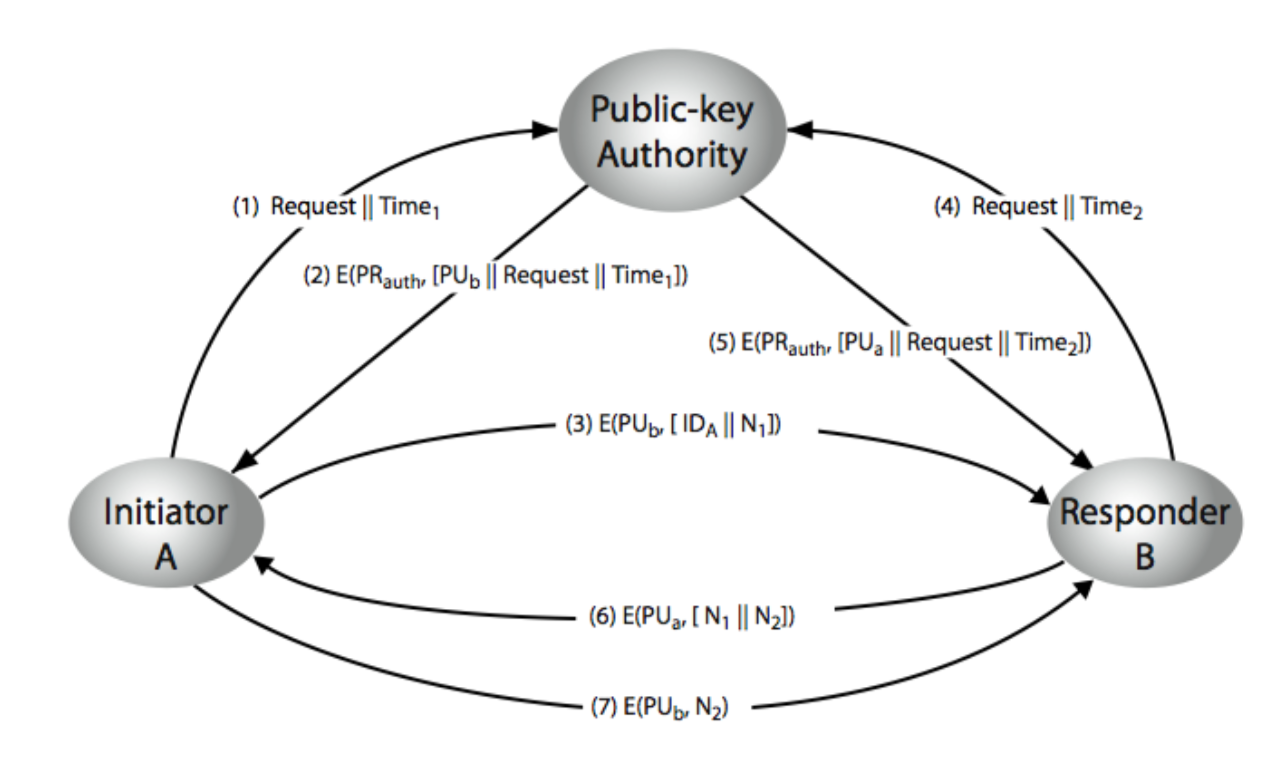
\includegraphics[width= 250pt]{pka.png}
\subsubsection{Public-key certificates}
\begin{itemize}
    \item allow key exchange without real-time access to PKA
    \item certificate binds identity to public key (usually with other info e.g. period of validity)
    \item all contents \textbf{signed} by a trusted PKA or Certificate Authority (i.e. Verisign)
    \item Can be verified by anyone who knows that PKA's public key
\end{itemize}
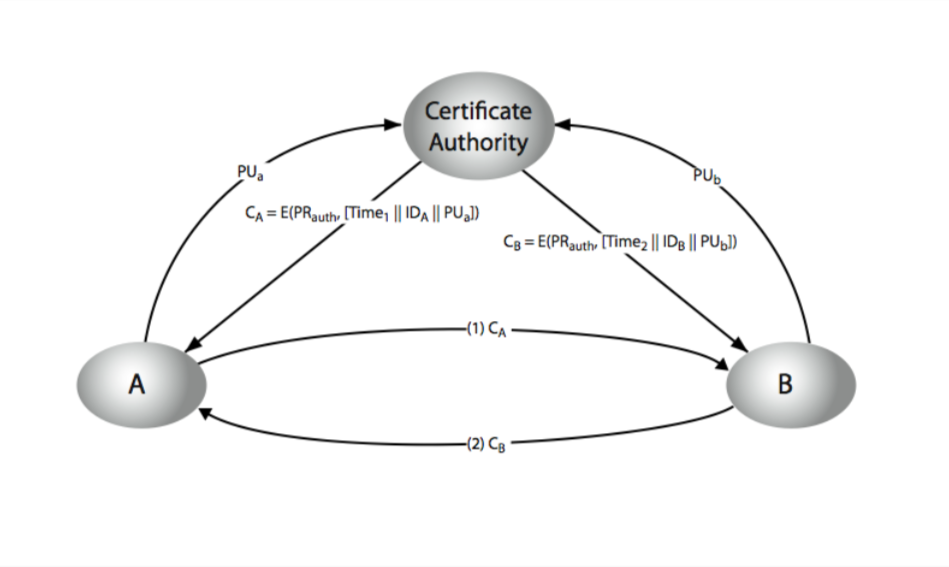
\includegraphics[width= 250pt]{ca.png}
\subsubsection{Public-key distribution of secret keys}
\begin{itemize}
    \item use previous methods to obtain public-key
    \item can use for secrecy or authentication
    \item but, public-key algorithms are slow
    \item usually we want symmetric key encryption to protect message contents, so we need a session key
    \item there are several alternatives for negotiating a suitable session
\end{itemize}
\subsubsection{Diffie-Hellman Key Exchange}
\begin{itemize}
    \item was the first public-key type scheme proposed by Diffie \& Hellman in 1976
    \item practical method for public exchange of a secret key
    \item used in a number of commercial products
    \item public key distribution scheme cannot be used to exchange an arbitrary message, but can be used to establish a common secret key between two participants
    \item key value depends on participants and their priv/pub key information
    \item based on exponentiation in a finite (Galois) field (modulo a prime or polynomial, easy)
    \item security relies on difficulty of computing discrete logarithms (similar to factoring) - hard
\end{itemize}
How do we set up D-H?
\begin{itemize}
    \item both users agree on global parameters: large prime int or polynomial $q$, $a$ being a primitive root modulo $q$
    \item $a$ and $q$ can be transmitted in the clear
    \item each user then generates their key, by choosing a secret key (number): $x_A < q$, and computing their \textbf{public key:} $y_A = a^{x_A} mod q$
    \item each user then publicises their $y_A$
    \item the shared session key for two users A and B is $K_{AB}$
    $$K = a^{x_A + x_B} mod q$$
    $$= y_{A}^{x_B} mod q$$ (which B can compute)
    $$= y_{B}^{x_A} mod q$$ (which A can compute)
    \item $K$ is used as a session key in symmetric encryption scheme between Alice and Bob
    \item attacker needs an $x$ (secret key), must solve discrete logarithm problem 
\end{itemize}
\section{Message Authentication}
\begin{itemize}
    \item sometimes we want to verify integrity/authenticity of message without needing confidentiality
    \item message authentication is the answer
    \item three ways: \textbf{message encryption}, \textbf{message authentication code (MAC)}, \textbf{hash function}
    \item we need authentication in these situations:
    \begin{enumerate}
        \item disclosure
        \item traffic analysis
        \item masquerade
        \item content modification
        \item sequence modification
        \item timing modification
        \item source repudiation
        \item destination repudiation
    \end{enumerate}
\end{itemize}
\subsection{Message Encryption}
Ciphertext of the entire message serves as its authenticator
\subsection{Message Authentication Code (MAC)}
A function of the message and a secret key that produces a fixed length value. This value serves as authenticator
\begin{itemize}
    \item generated by algorithm that creates a small, fixed-sized block
    \item algorithm depends on both message $M$ and some secret key $K$ such that $MAC = C(K,M)$, where $C$ is the MAC function
    \item similiar to encryption, but reversibility is not required (and often not implemented)
    \item appended to message to allow authentication
    \item receiver performs same computation on message and checks that it matches MAC, if so sender and integrity of message is verified
    \item we can also use MAC with encrypted messages using seperate keys for each process
    \item can encrypt message before or after MAC step (encrypting after protects against chosen ciphertext attacks, but more complex to implement)
    \item useful for when we only need authentication, even in longer term
    \item MAC is not digital signature: not unique. Many messages potentially have same MAC, but finding collisions assumed to be difficult
\end{itemize}
Requirements for MAC
\begin{enumerate}
    \item knowing a message and MAC, it is infeasible to find another message with the same MAC
    \item uniformly distributed: for $M$ and $M'$, probability that $C(K,M) = C(K,M')$ is $\frac{1}{2^n}$
    \item MAC should depend on all bits of the message equally
\end{enumerate}
We can also use symmetric ciphers for MACs.
\\e.g., we can use any block cipher chaining mode and then use the final block as the MAC
\\\textbf{Data Authentication Algorithm (DAA)} \textit{was} a popular MAC based on DES-CBC that used an IV of zero and a zero-pad of the final block. It encrypted message using DES-CBC, and sent just the final block (or leftmost $M$ bits \footnote{$16\leq M \leq 64$} of final block). However, this yields a final MAC that is too small to be secure
\section{Hashing Algorithms}
Hash functions transform messages of an arbitrary length to a fixed size $h = H(M)$. Hash functions are public, and typically \textbf{don't} use a key. We can compare hashes to detect changes to message. Most frequent applications of hashing are to create a digital signature for a file (e.g. \textbf{MD5}, \textbf{SHA})
\subsection{Requirements for hash functions}
\begin{itemize}
    \item can be applied to any size message $M$
    \item produces fixed-length output $h$
    \item is easy to compute $h = H(M)$ for any message $M$
    \item has one-way property: given $h$, infeasible to find $M$
    \item has weak collision resistance: given $x$, is infeasible to find $y$ such that $H(x) = H(y)$
    \item has strong collision resistance: infeasible to find an $x,y$ pair such that $H(x) = H(y)$
\end{itemize}
\subsection{Simple Hash Functions}
several proposals for simple functions, based on XOR of message blocks
\\Message is arranged into ~$ \frac{m}{n} $ blocks, where $m$ = message length and $n$ = hash size
\\RXOR (rotate XOR), generally not crypotographically secure
\subsection{Secure Hash Algorithm (SHA)}
\begin{itemize}
    \item originally designed by NIST and NSA in 1993
    \item revised as SHA-1 in 1995
    \item US standard for use with DSA signature scheme (FIPS 180-1 1995, RFC3174)
    \item based on MD4 but with some differences (produces 160-bit hash values)
    \item SHA-1 is no longer considered secure, SHA2 recommended
\end{itemize}
\subsection{In summary}
\begin{itemize}
    \item Hash Functions
    \begin{itemize}
        \item condense arbitrary size message to fixed size by processing message in blocks through some unkeyed compression function
    \end{itemize}
    \item Message Authentication Code (MAC)
    \begin{itemize}
        \item fixed size authenticator for some message using either block cipher mode or keyed hash
    \end{itemize}
\end{itemize}
\section{Introduction to Secure SHell (SSH)}
\subsection{What is SSH?}
\begin{itemize}
    \item SSH provides secure channel over unsecured network in client-server architecture
    \item SSH client connects to SSH server
    \item provides Confidentiality and Integrity, with authentication
    \item SSH-1 and SSH-2 versions
\end{itemize}
\subsection{Overview}
There are two phases to SSH
\begin{itemize}
    \item session key generation
    \item public-key based authentication (optional)
\end{itemize}
SSH uses several crypto primitives:
\begin{itemize}
    \item chacha20-poly1305
    \item aes128-ctr
    \item aes256-ctr
    \item aes128-gcm
    \item aes256-gcm
    \item aes128-cbc
    \item aes192-cbc
    \item aes256-cbc
    \item 3des-cbc
    \item Diffie-Hellman key exchange
    \item HMAC (hashed MAC)
\end{itemize}
\subsection{Session Key Generation}
\begin{enumerate}
    \item TCP handshake
    \item SSH handshake begins
    \item client shares crypto algorithms it can support
    \item server agrees on one of them
    \item client and server begin DH key exchange and generate a session key
    \item each message must contain a MAC to verify packet integrity
    \begin{itemize}
        \item this MAC is calculated from the shared secret, the packet seq\#, and the actual message contents
    \end{itemize}
\end{enumerate}
\subsection{User authentication}
\begin{itemize}
    \item password-based (encrypted with session key)
    \item public-key based (recommended!)
    \begin{itemize}
        \item user sends public key to server
        \item it is saved in ~/.ssh/authorised\_keys file serverside
        \item now user can log in without password, using their private key to authenticate
    \end{itemize}
\end{itemize}
\section{Introduction to Secure Sockets Layer (SSL)}
\subsection{Problems in web security}
\begin{itemize}
    \item Confidentiality
    \begin{itemize}
        \item eavesdropping on connections
        \item theft of info from server or client
        \item solution: \textbf{encryption}
    \end{itemize}
    \item Integrity
    \begin{itemize}
        \item modification of user data
        \item trojan horse browser
        \item modification of memory
        \item modification of message traffic in transit
        \item solution: \textbf{cryptographic checksums}
    \end{itemize}
    \item Authentication
    \begin{itemize}
        \item Impersonation of users
        \item data forgery
        \item solution: \textbf{cryptographic signatures}
    \end{itemize}
    \item Location of the threat:
    \begin{itemize}
        \item web server
        \item web browser
        \item network traffic
    \end{itemize}
\end{itemize}
\subsection{What is SSL?}
\begin{itemize}
    \item \textbf{transport layer} security service
    \item developed by Netscape originally, v3 with public input
    \item subsequently became internet standard known as TLS (transport layer security)
    \item uses TCP for reliable service
    \item has two layers of protocols
    \begin{enumerate}
        \item L1: SSL Record Protocol
        \item L2: Handshake, change cipher, alert
    \end{enumerate}
    \item Handshake for session init, record for data transfer, alert for message passing, change cipher for changing crypto method
\end{itemize}
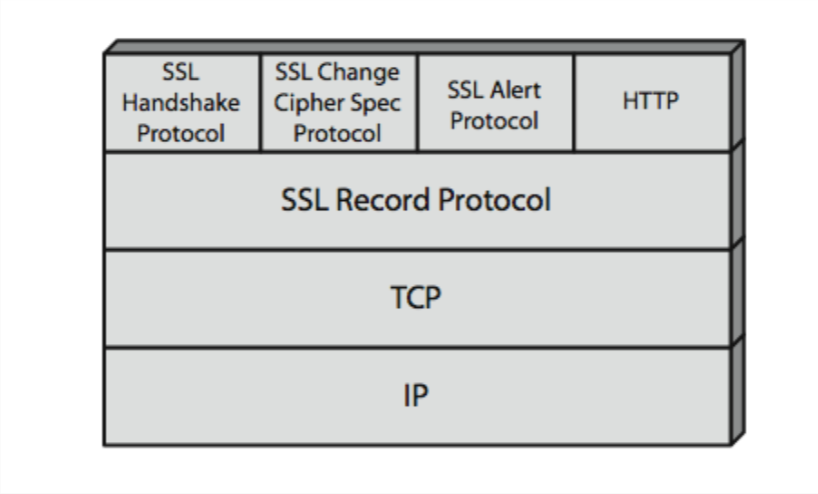
\includegraphics[width= 250pt]{sslstack.png}
SSL Connection:
\begin{itemize}
    \item transient, p2p communications link associated with 1 SSL \textbf{session}
    \item Dimensions:
    \begin{itemize}
        \item server and client random byte
        \item server write MAC secret: secret key for MAC
        \item client write MAC secret: secret key for MAC
        \item server write key: encryption key
        \item client write key: encryption key
        \item init vectors
        \item sequence numbers for packets
    \end{itemize}
\end{itemize}
SSL Session:
\begin{itemize}
    \item association between client and server
    \item created by handshake protocol
    \item \textbf{defines} a set of cryptographic parameters
    \item may be shared by \textbf{multiple} SSL connections
    \item Dimensions:
    \begin{itemize}
        \item session identifier generated by server
        \item peer certificate (X.509 v3)
        \item compression method
        \item cipher specification
        \item master secret
        \item is resumable?
    \end{itemize}
\end{itemize}
\subsection{SSL Record Protocol Services}
\begin{itemize}
    \item message integrity: using a MAC with a shared secret key, similar to HMAC but with some differences
    %maybe include code snippet here? lecture9slide11
    \item confidentiality: use symmetric encryption with a shared secret key defined by handshake protocol
    \item AES, IDEA, RC2-40, DES-40, DES, 3DES, Fortezza, RC4-40, RC4-128
    \item message is optionally compressed before encryption
\end{itemize}
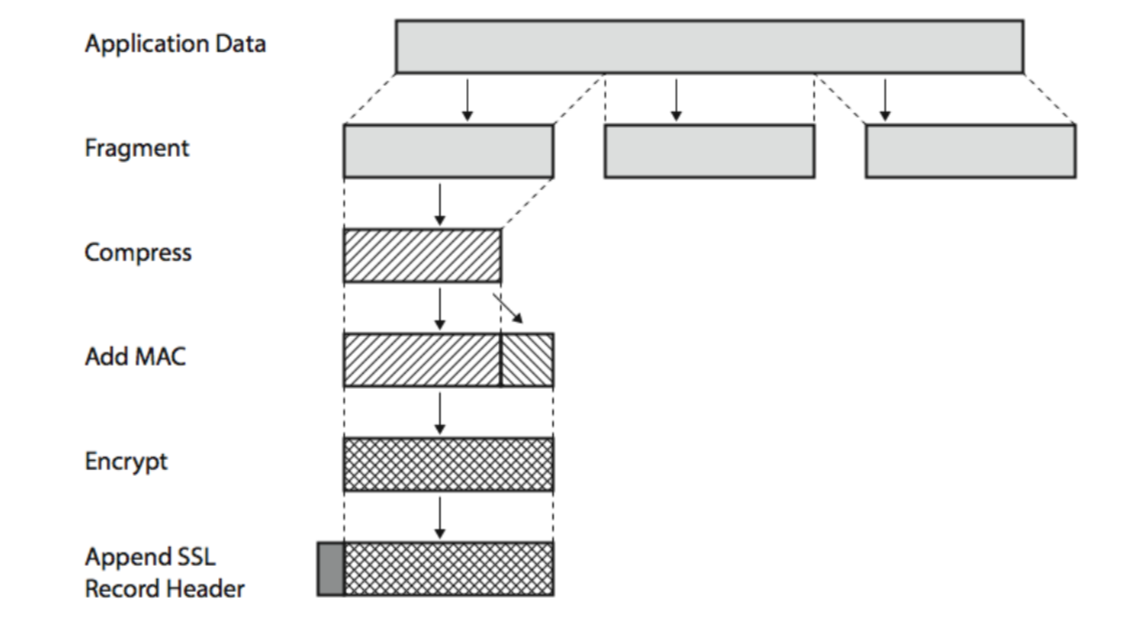
\includegraphics[width= 250pt]{sslblock.png}
\subsection{SSL Change Cipher Spec Protocol}
\begin{itemize}
    \item one of 3 SSL specific protocols which use the SSL record protocol
    \item single message consists of just one byte: 1
    \item causes pending state to become current, updating cipher suite in use
    \item sent after just-negotiated cipherspec and keys
\end{itemize}
\subsection{SSL Alert Protocol}
\begin{itemize}
    \item conveys SSL-related alerts to peer entity
    \item 2 byte messages
    \item severity indicated in the first byte (warning or fatal)
    \item specific alert in the second byte
    \begin{itemize}
        \item fatal: unexpected message, bad record mac, decompression failure, handshake failure, illegal parameter
        \item warning: close notify, no cert, bad cert, unsupported cert, cert revoked, cert expired, cert unknown
    \end{itemize}
    \item compressed and encrypted like all SSL data
\end{itemize}
\subsection{SSL Handshake Protocol}
\begin{itemize}
    \item allows server and client to: authenticate eachother, negotiate encryption and MAC algorithms and negotiate crypto keys to be used
    \item comprises of a series of messages in phases
    \begin{enumerate}
        \item establish security capabilities
        \item server authentication and key exchange
        \item client authentication and key exchange
        \item finish
    \end{enumerate}
\end{itemize}
Format of these messages
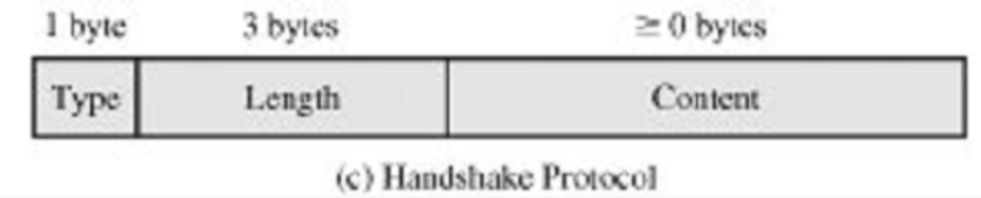
\includegraphics[width= 250pt]{sslHP.png}
\begin{itemize}
    \item Type (1 byte): indicates one of 10 messages
    \item Length (3 bytes): the length of the message in bytes
    \item Content ($\geq0$ bytes)
\end{itemize}
\subsection{Transport Layer Security (TLS)}
IETF standard RFC 2246 similiar to SSLv3, but with minor differences
\begin{itemize}
    \item record format version number is different
    \item uses HMAC for MAC
    \item a pseudo-random function expands secrets
    \item has additional alert codes
    \item some changes in supported ciphers
    \item changes in cert types and negotiations
    \item changes in crypto computations and padding strategy
\end{itemize}
\section{Systems Security}
\textbf{Computer Security:} Prevent attackers from doing things with unauthorised access to computers and/or networks
\\\textbf{Programmer:} make sure source code is correct, secure and performs well
\\\textbf{System integrator:} responsible for integrating new and existing software to create programs or systems to satisfy customer requirements
\\\textbf{Sysadmins:} responsible for managing and securing one or more systems. Installing, updating and removing software and managing system privileges
\\\textbf{Network Admins:} manage (secure) network operations
\\\textbf{Security Analyst:} concerned with properties of security flaws and how to identify them
\\\textbf{Vulnerability Analyst:} analyses vulnerablities in existing programs
\\\textbf{Security Researcher:} develops exploits and mitigation strategies for those exploits
\\\textbf{Attacker:} malicous, exploits vulnerabilities to achieve a goal. These goals vary depending on threat
\\\textbf{Security Policy:} A set of rules and practices that specify how an organisation or system secures sensitive and critical (system) resources
\\\textbf{Software defect:} encoding of human error in software
\\\textbf{Security flaw:} software defect that poses a \textbf{security risk}. If we eliminate software defects, we can eliminate security flaws
\\\textbf{Weakness:} a type of behaviour that has potential to allow an attacker to violate a security policy if the behaviour is accessible to the attacker
\\\textbf{Vulnerability:} set of conditions that allow an attacker to violate an explicit or implicit security policy. Not all security flaws lead to vulnerabilities, but they can cause a program to be vulnerable. Vulnerabilities can exist without a security flaw (i.e., Rowhammer uses a physical vulnerability). Composed of one or more (related) weaknesses that allow an actor to access things that would otherwise be inaccessible to them. Intersection of three elements: system flaw, attacker access to flaw, attacker capability to exploit flaw.
\\\textbf{Exploit:} piece of software or a technique that takes advantage of a vulnerability to violate an explicit/implicit security policy. Failed exploits could crash software/a system. Proof-of-concept exploits are developed to prove existence of vulnerability, and are beneficial so long as they don't leak/fall into wrong hands.
\\\textbf{Mitigation:} methods of preventing or limiting exploits, protecting against vulnerabilities. Can range from code improvements to infrastructure changes (e.g. not using strcpy to closing ports on router)

\subsection{Vulnerability Detection}
Automated detection is an unsolved problem, but there are approaches to try and approximate this
\begin{itemize}
    \item \textbf{taint analysis:} track user data through program and see whether it passes through dangerous places
    \item \textbf{Fuzzing:} test the program with lots of inputs at program and see if one breaks it/exposes a vulnerability
\end{itemize}
The above approaches are incomplete at best
\subsection{C and C++}
\begin{itemize}
    \item popular
    \item composes vast majority of reported vulnerabilities
    \item does not protect programmers. problems arise from poor understanding of how abstractions translate to machine instructions
    \item no type safety, doesn't protect against things like writing over the boundaries of an array
    \item Legacy code written before mainstream standardization of C is still pervasive, and is at higher risk for security flaws because of looser compiler standards
\end{itemize}
\textbf{Short term solutions}
\begin{itemize}
    \item educate developers to program securely and apply appropriate mitigations
\end{itemize}
\textbf{Long term solutions}
\begin{itemize}
    \item language standard, compilers and tools evolve
    \item replace these languages? Unlikely to happen, system software relies on high performance of these languages
\end{itemize}
Adopting languages like Java not viable because of:
\begin{itemize}
    \item existing investment in C
    \item programming expertise
    \item development environments
    \item performance (java can have a lot of overhead)
    \item closeness to hardware allows for better performance
\end{itemize}
\subsection{Typical Memory Layout of a program}
Windows PE and Linux ELF file formats
\\Main segments of binary program:
\begin{itemize}
    \item executable code (text/code)
    \item initialized data (data)
    \item uninitialized data (bss)
    \item heap (dynamic memory allocation)
    \item executed code and data of needed shared libraries (dynamically loaded into the space)
    \item program stack (temporary storage used by functions)
\end{itemize}
\section{Application Security}
\subsection{Assembly}
\begin{itemize}
    \item low-level symbolic language
    \item processor-specific due to availability of instructions
    \item directly translated into machine language
    \item we focus on \textbf{user-mode x86-64 assembly} which is used by most PCs
    \item We use AT\&T syntax for assembly (intel swaps param order)
\end{itemize}
Program composed of:
\begin{itemize}
    \item instructions
    \item directives: assembler commands
    \item labels: create symbol at current address
    \item comments: text after \# is ignored
\end{itemize}
Assembly instructions:
\begin{itemize}
    \item general form of \textit{mnemonic source, destination} (in AT\&T syntax)
    \item \textbf{mnemonic} is a shortcode telling cpu what to do e.g. mov, jump
    \item source and destination are operands. They can be \textbf{registers}, \textbf{memory addresses}, or \textbf{constants} (for source arguments: obviously a destination cannot be a constant)
    \item the number and type of operands varies per instructions. There may be fewer operands than two and (rarely) may be more. Operands may be implicit. At most one explicit memory operand is allowed.
\end{itemize}
\subsubsection{Registers}
\begin{itemize}
    \item memory locations on CPU itself
    \item general purpose (\verb|\%rax, \%rbx, \%rcx, \%rdx, \%rsi, \%rdi, \%r8-\%r15|)
    \item stack pointer \verb|\%rsp|
    \item frame pointer \verb|\%rbp|
    \item instruction pointer \verb|\%rip|
    \item flags register
    \item segment registers, rarely used in 64-bit
    \item system registers, only used in kernel
    \item instruction set registers, only used with special instructions
\end{itemize}
Default registers are 64-bit, but smaller parts can be used if the whole 64-bits is not necessary
\\Setting 32-bit sub registers clears the other bits, but setting smaller sub-registers retains the other bits
\subsubsection{Memory}
\begin{itemize}
    \item memory is accessed by \textbf{dereferencing} pointers
    \begin{itemize}
        \item \textit{displacement(base, index, scale)}
        \item refers to \textit{displacement+base+index*scale}, where base and index are 64-bit registers and displacement is a 32-bit constant or symbol (default = 0)
        \item scale = 1, 2, 4,or 8 (default = 1)
        \item all parts are optional
        \item alternatively, base can be \verb|\%rip| (address of next instruction) if index is omitted, in which case sumbolic displacement will be relative to that address
    \end{itemize}
    \item Operand size specified as suffix to mnemonic
    \begin{itemize}
        \item b for byte, w for word (16-bits), l for long (32-bits) q for quad (64 bits)
        \item optional if other operand is a register
    \end{itemize}
\end{itemize}
\subsection{Endianess and Signed integers}
\begin{itemize}
    \item Intel uses little endian ordering
    \item signed integers expressed in twos complement notation
    \item sign is changed by flipping bits and adding one, ignoring overflow
\end{itemize}
\subsubsection{Common Instructions}
\textbf{Data transfer:}
\\\verb|mov src, dest| dst = src
\\\verb|xchg dst1, dst2| swap dst1 and dst2
\\\verb|push src| store src on top of stack
\\\verb|pop dst| retrieve top of stack into dst
\\\textbf{Binary Arithmetic:}
\\\verb|add src, dst| dst += src
\\\verb|sub src, dst| dst -= src
\\\verb|inc dst| dst++
\\\verb|dec dst| dst--
\\\verb|neg dst| dst = -dst
\\\verb|cmp src1, src2| set flags based on the result of src2 - src1
\\\textbf{Logical}
\\\verb|and src, dst| dst \&= src
\\\verb|or src, dst| dst |= src
\\\verb|xor dst, src| dst $^ =$ src
\\\verb|not dst| dst = $\tilde{}$ dst
\\\verb|test src1, src2| set flags based on src1 \& src2
\\\textbf{Unconditional Branches}
\\\verb|jmp addr| jump to addr
\\\verb|call addr| push return address to stack, then call function (at) addr
\\\verb|ret| pop return address and return there 
\\\verb|syscall| enter the kernel to perform a system call
\\\textbf{Miscellaneous}
\\\verb|lea src, dst| dst = \&src (src must be in memory)
\\\verb|nop| do nothing

\subsubsection{Conditional Branches}
general form: \verb|jcc addr|
\\jumps to addr only if condition cc holds, decided using flags register which is implicitly set by arithmetic and logical instructions
\textbf{Common choices for condition code cc}
\begin{itemize}
    \item e/z equal/zero result = 0
    \item b below dst $<$ src (unsigned)
    \item a above dst $>$ src (unsigned)
    \item l less dst $<$ src (signed)
    \item g dst $>$ src (signed)
    \item s sign result $<$ 0 (signed)
    \item ncc not test for opposite condition
\end{itemize}
\subsubsection{Data definition}
Data objects defined in a data segment using syntax
\\\verb|label:      .type        data1, data2, ...|

\subsection{Stack Frames}
\subsubsection{The stack}
The stack grows towards \textbf{lower memory addresses}, with stack pointer \verb|\%rsp| pointing to top of stack
\\The stack is composed of \textbf{frames}, which are pushed onto the stack as a consequence of a function call. The address of the current frame is stored in the frame pointer (FP) register, which is \verb|\%rbp| on intel architectures.
\\Each frame contains:
\begin{itemize}
    \item the functions actual parameters if they are not in registers
    \item the return address to jump back to at the end of the function
    \item the pointer to the previous frame
    \item the functions local variables
\end{itemize}
\textbf{Compiler optimization may eliminate stack frames!}
\subsubsection{Parameter passing in caller function}
(In Linux, specifically)
\begin{itemize}
    \item Before calling a function, caller prepares params by either setting specific registers or pushing them to stack (so they are not lost when new stack elements are pushed if they are top of stack)
    \item Store as many ints, pointers and small structs as possible in registers. The following registers are used for this from left to right: \verb|\%rdi \%rsi, \%rdx, \%rdx, %\r8, \%r9|
    \item most other params (with the exception of floats) are pushed onto the stack from right to left
\end{itemize}
\subsubsection{Prologue in calling function}
\begin{itemize}
    \item push the old base pointer onto the stack \verb|\%rbp|
    \item set the base pointer to be the current stack pointer \verb|\%rsp|
    \item move the stack pointer to make room for local variables
    \item we have an \verb|enter| opcode for these operations, but it does \textbf{not} push preserved registers
\end{itemize}
\subsubsection{Epilogue in calling function}
\begin{enumerate}
    \item save the result (if there is one) in \verb|\%rax|
    \item restore old stack pointer from base pointer, deleting current stack frame
    \item restore registers that must be preserved for the caller from the stack
    \item restore base pointer from stack
    \item executes a \verb|ret|
    \item \verb|leave| opcode is a shorthand for operations two and four, but does \textbf{not} restore preserved registers
\end{enumerate}
\section{Exploitation Techniques in Application Security}
\subsection{Buffer Overflows}
\begin{itemize}
    \item lack of boundary checking is one of most common mistakes in C/C++
    \item as a result, bufferoverflows are among the most popular attacks, as they can be exploited both locally and remotely and can modify data flow and control flow of application
    \item recent tools make exploiting buffer overflows easy, if not automatic
    \item lots of research has been put into developing prevention techniques and detection mechanisms
\end{itemize}
\textbf{The buffer overflow attack family}
\begin{itemize}
    \item stack-based
    \begin{itemize}
        \item shellcode injection
        \item return into libc
        \item return-oriented programming (ROP)
    \end{itemize}
    \item heap-based overflows
    \item integer overflows
    \item user-controlled format strings
\end{itemize}
\subsection{Stack-based overflows and shellcode}
\begin{itemize}
    \item data copied without checking boundaries
    \item overflows pre-allocated buffer, overwriting return address, \textbf{normally} causing a segfault
    \item If correctly crafted, possible to overwrite return address with user-defined value, and possibly jump to user-defined code (i.e. code that invokes a shell)
    \item the code may be part of the overflowing data, or not, and the code will be executed with the privileges of the running program (which makes system level exploits \textit{really} bad)
\end{itemize}
\textbf{Overflowing Functions}
\begin{itemize}
    \item \verb|gets()|
    \item \verb|strcpy(), strcat()|
    \item \verb|sprintf(), vsprintf(), scanf(), sscanf(), fscanf()|
    \item and also, some custom input routines
\end{itemize}
\subsubsection{Guessing the buffer address}
\begin{itemize}
    \item in most cases, the address of the buffer is not known, and has to be very precisely guessed
    \item we can use a dummy program to roughly guess stack address of a program, and then assuming the same environment and knowing the size of the parameters, we can roughly guess the address of the stack
    \item also have to guess offset of the buffer w.r.t the stack pointer
\end{itemize}
\textbf{NOP Sled:} Use a series of NOPs at the beginning of the overflowing buffer so that the jump does not need to be too precise
\subsubsection{Return Oriented Programming (ROP)}
\begin{itemize}
    \item modern defenses protect against (traditional) stack smashing
    \item Data Execution Prevention (DEP) prevents executing writable memory, and ASLR (Address Space Layout Randomization) randomises location of memory (stack, heap, libraries etc)
    \item executables often not position-independent, so we can reuse code from the executable itself by collecting operations (gadgets) that do a small operation followed by a return and chain them all together
\end{itemize}
\subsubsection{Overwriting Values on the Stack}
\begin{itemize}
    \item Stack-based buffer overflows affecting return address of a function are obvious source of problems
    \item any reference to an overwritable value can be a vulnerability. Pointers to strings can have their value changed, as well as integers.
    \item Changing value of saved base pointer in order to force a process to use a function frame chosen by the attacker when returning from a function, with an additional return operation that could jump to a destination selected by the attacker
    \item change the value of a function pointer
\end{itemize}
\subsection{Other Attacks}
\begin{itemize}
    \item Longjmp overflows: overflow information in that setjmp() stores to jump to arbitrary code
    \item Array overflows: exploit code that uses user-provided input as an index in an array, without checking boundaries. Can allow for direct assignment of memory values
    \item Off-by-one overflows: exploit situations in which only a single byte can be overwritten
    \item Non-terminated string overflow: if a string under the attackers control is not null-terminated, a subsequent \verb|strcpy()| may cause an overflow. If adjacent buffers are all not null-terminated, strcpy() will copy more than it is intended to and overflow a buffer
    \item Integer overflows: Exploit inadequate size and/or signedness of integer values (truncation, arithmetic overflow, signedness)
    \item Dangling Pointers: variables can be overwritten without buffer overflow if they are used after being freed, as the pointer may be kept by the program
    \item Uninitialized variables: It can be possible to manipulate the contents of uninitialised variables, as C doesn't automatically initialise them. They contain whatever was at that address at the time of creation
    \item \verb|data| and \verb|bss| overflows: variables and function pointers in data and bss segments can be the target of a buffer overflow attack
    \item Format string vulnerability: using user-supplied input, it is possible to write arbitrary values to process memory with a carefully crafted format string, as well as leak values from the register/stack using string formatting. Can thus overwrite bytes using an existing pointer, or using an attacker-controlled pointer.
\end{itemize}
\subsection{Heap Overflows}
Heap is area of memory dynamically allocated through the \verb|malloc()| family of functions
\\Memory allocated on the heap outlasts the function that created it.
\\Heap grows towards \textbf{higher memory addresses}
\\Memory management done through in-band control structures, which can be manipulated by heap overflows to execute arbitrary code
\\Arch/OS dependent
\\Some attacks depend on library used to manage the heap

\section{Simple Attacks in Application Security}
\subsection{Application Security}
\begin{itemize}
    \item Applications provide services 
    \begin{itemize}
        \item Locally
        \item Remotely
    \end{itemize}
    \item Behaviour of an application is determined by
    \begin{itemize}
        \item code being executed
        \item data being processed
        \item environment in which application runs
    \end{itemize}
    \item Attacks force applications to violate system security
    \begin{itemize}
        \item violation of integrity
        \item violation of confidentiality
        \item violation of availability
    \end{itemize}
\end{itemize}
\subsubsection{Application Vulnerability Analysis}
\begin{itemize}
    \item Identifying vulnerabilities in applications
    \item Deployment vulnerabilities, i.e:
    \begin{itemize}
        \item Installed with unnecessary privileges
        \item faulty security policies (i.e. a file that only needs to be read is also writable)
    \end{itemize}
    \item Implementation vulnerabilities
    \begin{itemize}
        \item unexpected input
        \item unexpected errors/exceptions
        \item unexpected interleaving of events
    \end{itemize}
\end{itemize}
\subsubsection{Local and Remote Attacks}
\begin{itemize}
    \item \textbf{Local attacks}
    \begin{itemize}
        \item manipulate behaviour of an application through local interaction
        \begin{itemize}
            \item requires a previously established presence on host (e.g. an account or existing malware deployed)
        \end{itemize}
        \item allow one to execute operations with privileges that are different (usually superior) than what an attacker would otherwise have
        \item are easier to perform, because attacker has better knowledge of host environment
    \end{itemize}
    Each process in Unix has three UID/GID pairs. Real IDs for the user who started/owns process, Effective IDs (whose permissions should we check), and Saved IDs (used to regian previously dropped privileges). The SUID bit can set the effective UID/GID to the program files owner when executed. Most \textbf{local} vulnerabilities exploit SUID-root programs to gain root privileges, and from there can target the OS itself.
    \item \textbf{Remote attacks}
    \begin{itemize}
        \item manipulate behaviour of an application through network-based interaction
        \begin{itemize}
            \item unauthenticated remote attacks: interaction with application does not require authentication of prior capabilities 
        \end{itemize}
        \item Allow one to execute operations with privileges of vulnerable application
        \item are more difficult to perform but also more powerful, as they do not require prior access to the system
    \end{itemize}
\end{itemize}
\subsection{Simple Attacks}
\begin{itemize}
    \item environment attacks
    \item input arguments attacks
    \item file access attacks
    \begin{itemize}
        \item race condition attacks
        \item file descriptor attacks
    \end{itemize}
\end{itemize}
\textbf{Invoking external programs}
\begin{itemize}
    \item applications invoke external commands to carry out specific tasks
    \item execution of these external commands can be influenced by the environment
    \item HOME and PATH variables in the environment can be modified to change the behaviour of these external commands/ cause them to execute other commands
\end{itemize}
\textbf{Playing with command line parameters}
Often used by applications without size checking or sanitation
\\User provided data can be used to perform:
\begin{itemize}
    \item command injections (; attack)
    \item unexpected options to commands
    \item directory traversal attacks (.. attack)
\end{itemize}
Command line params should always be checked for length/size if copied into local buffers, and should \textbf{always} be sanitized. 
\\In general, escape possibly dangerous input. Instead of denying things that aren't allowed, decide what \textbf{is} allowed and deny \textbf{everything} else.
\\Also applies to web based input, SQL etc.
\textbf{Playing with the file system}
many applications create/use temporary files for logging, locking. Some do not test whether the file already exists, or whether the file is actually a symlink. An attacker could create a symbolic link to a file accessible only to a superuser and then invokes the application.
\textbf{Time Of Check To Time Of Use (TOCTTOU attack)}
Attacker may race against application by exploiting the gap between testing and accessing the file
\begin{itemize}
    \item Time-Of-Check ($t_1$): validity of assumption A on entity E is checked
    \item Time-Of-Use ($t_2$): E is used, assuming A is still valid
    \item Time-Of-Attack ($t_3$): assumption A is invalidated
    \item $t_1 < t_3 < t_2$
\end{itemize}
Data race condition: conflicting accesses of multiple processes to shared data, with at least one of them being a write access.

\subsection{To summarise}
\begin{itemize}
    \item verify/validate assumptions made about file system
    \item Use truly random filenames
    \item Preventing TOCTTOU race conditions
    \begin{itemize}
        \item Use versions of system calls that use file descriptors instead of file path names
        \item Perform file descriptor binding first
    \end{itemize}
\end{itemize}

\section{Real World Security: We all make mistakes}
\subsection{Writing good (and secure) code}
\begin{itemize}
    \item Threat modelling:
    \begin{itemize}
        \item Identify what threats are posed
        \item Identify who that threat affects
        \item Identify how these threats to these objects can be mitigated
    \end{itemize}
    \item Code reviews: other people might notice things you missed
    \item Compiler warnings (use lots of compiler flags to hit small stuff)
    \item Static code analysis (i.e. in C++ you can use cppcheck)
    \item In C you can use Valgrind to check memory safety
    \item Fuzzing: test your program with a variety of inputs (even inputs that you wouldn't expect)
    \item Sanitizers for both addresses and memory to prevent use-after free vulnerabilities or memory leaks
    \item Mitigations
    \begin{itemize}
        \item Also known as hardening
        \item Can be done automatically by the compiler, runtime and/or kernel
        \item Makes it \textbf{more difficult} to exploit a vulnerability, but doesn't fix the vulnerability
    \end{itemize}
\end{itemize}
\subsection{Detecting and stopping exploitation}
\begin{itemize}
    \item We can use Stack Canaries (just a placeholder stack item) to detect when too much of a stack is being read
    \item We can also use Stack Cookies to detect and help prevent buffer overflows
    \item Check for integer overflows and use bounds checking to make sure you avoid overflows
\end{itemize}
\subsection{Preventing an attacker from executing malicious code}
\begin{itemize}
    \item We can prevent execution of arbitrary code on the stack by marking things on the stack as \textbf{non-executable}, using \textbf{Data Execution Prevention (DEP)}.
    \item DEP also prevents execution from the Heap as well.
    \item DEP can be countered by using "Return to libc"
    \begin{itemize}
        \item Use snippets from existing code by pushing return addresses and parameters to the stack that point to the target instructions
        \item a NOP (No execution OPeration) sled can be used to execute a specific instruction, as whatever memory address a program branches to, it will end up on that target instruction as long as that memory address is on the sled.
    \end{itemize}
    \item Address Space Layout Randomization (ASLR)
        \begin{itemize}
            \item Memory is typically assigned starting from lower addresses to higher, in blocks
            \item This is ideal for an attacker, as the locations of certain things in memory can be approximated
            \item With ASLR, we randomize all of these addresses, so that the order of objects in memory is arbitrary, meaning it is much harder to approximate the location of a variable in memory
            \item Pointers can leak the location of objects even with ASLR, effectively rendering it useless if this attack vector is used
        \end{itemize}
\end{itemize}
\subsection{Exploitation isn't necessarily impossible, even with all of the software patches}
\begin{itemize}
    \item ASLR addresses can be leaked by the MMU, even by javascript in the browser
    \item Rowhammer can be used to flip bits at a hardware level by writing to specific memory cells repeatedly. This attack can be used in a wide variety of ways
\end{itemize}

\section{Web Security}
The Web is a powerful platform for developing and distributing applications, built on a mix of client and server-side components. The aim is for the platform to be open, with documents and data on the client-side are always visible and writable. However, web apps are vulnerable. Because they are popular, they are an attractive target for many attackers. Sensitive data is typically available on the server-side, increasing the appeal for many attackers.
\subsection{The Web Model}
\begin{itemize}
    \item HyperText Markup Language (HTML) as a markup language for arranging content
    \item HyperText Transfer Protocol (HTTP) designed for downloading HTML documents, but can also be used for downloading other files
    \item HTTP offers basic authentication, but user credentials are only encoded, not encrypted. Easily reversible
\end{itemize}
\subsubsection{Cookies}
\begin{itemize}
    \item Basic mechanism to ensure a persistent state as you browse
    \item Allows services to store small amounts of data with the client, used for identification, authentication and tracking
    \item Domain and path of a cookie restricts the resources a browser will send cookies to, with expiration dates determining how long a browser should keep a cookie
    \item There are some additional security restrictions baked into cookies too
    % look at me go with this shitty joke
    \item Cookies are manipulated by \verb|Set-Cookie| and \verb|Cookie| request and response headers.
\end{itemize}
\textbf{A typical Session Cookie lifecycle}
\begin{enumerate}
    \item Client submits login credentials
    \item App validates credentials
    \item App generates and stores a cryptographically secure session ID, which is hashed and encoded (e.g. \verb|HMAC(session_id)|
    \item App uses \verb|Set-Cookie| to set the session ID
    \item Client sends the session ID as part of subsequent requests using Cookie
    \item Session is dropped by either the expiration of the cookie or the removal of the servers record of the session
\end{enumerate}
\textbf{Advantages of Session Cookies}
\begin{itemize}
    \item Flexible: authentication is delegated to the App layer (vs what HTTP authentication offers)
    \item Supports logging out, as you can expire the cookie or the session record on-demand
    \item There are a large number of ready-made session management frameworks available
\end{itemize}
\textbf{Disadvantages of Session Cookies}
\begin{itemize}
    \item Authentication is delegated to the App layer
    \item Session security depends on secrecy, unpredictability and tamper-evidence of cookie, not guaranteed when the user can modify them
\end{itemize}
\textbf{Managing Cookie States}
\begin{itemize}
    \item Each origin may set cookies, with objects from embedded resources also being able to
    \item Only cookies for the origin of a HTTP request are included in a HTTP request (assuming they obey the specified path constraints)
\end{itemize}
\subsubsection{Same Origin Policy (SOP)}
\begin{itemize}
    \item States that subjects from one origin cannot access objects from another, the basis of "classic" web security
    \item SOP has been relaxed over time to make controlled sharing easier
    \item JS from origin D cannot access objects from origin E, but JS \textit{included} in D can access all objects in D
\end{itemize}
In the case of cookies: domains are the origins, and cookies are the subjects.
\textbf{JavaScript and the Document Object Model (DOM)}
JavaScript is a scripting language that can be used to manipulate objects in a HTML page without having to manually refresh the page or rewrite the code. It's modifications are not permanent.
\\Should JavaScript from one domain be able to access objects in other domains?
\textbf{CSS}
CSS is used for styling, not super exploitable but some browsers do allow for JS inside CSS, and will execute JS used in this way, so watch out for that.
\subsubsection{XMLHttpRequest (XHR)}
\begin{itemize}
    \item Provides an API for asynchronous network requests in JavaScript
    \item This API is browser specific, and often abstracted away by a library (e.g. jQuery)
    \item SOP restrictions still apply, with some exceptions to be discussed later
    \item Typical workflow:
        \begin{enumerate}
            \item Handle a client-side event (like a button click)
            \item Invoke an XHR to the server
            \item Load the resulting data from the server (HTML, XML, JSON)
            \item Update the DOM with this new information
        \end{enumerate}
\end{itemize}
With XHR, requests to objects from the same origin are legal. However, requests for objects from other origins aren't legal.
\subsubsection{Sending Data over HTTP}
There are four different ways to achieve this
\begin{enumerate}
    \item Embedded in the URL (usually, but not always, URL encoded)
    \item In cookies (cookie encoded)
    \item Inside a custom HTTP request header
    \item In the HTTP request body (form-encoded)
\end{enumerate}

\subsection{Attacking Web Clients}
\subsubsection{Focussing on the client}
It also makes a lot of sense for an attacker to attempt to attack a client:
\begin{itemize}
    \item Your browser stores a lot of information (your history, saved usernames, passwords, payment details, and (session) cookies)
    \item Browsers are obviously designed to protect this information as best as they can, but that doesn't make them exempt from vulnerabilities
\end{itemize}
We can create a threat model for the web:
\begin{itemize}
    \item Attacker's goal
        \begin{itemize}
            \item steal information from your browser
            \item Execute arbitrary code in your browser (i.e. crypto mining)
            \item Execute arbitrary code to exploit your browser, allowing it to drop malware into your system
        \end{itemize}
    \item Browser's goal
        \begin{itemize}
            \item Prevent attacker from stealing your private information
            \item Preventing code injection attacks is up to the server, not the client (as it may be the intention that the browser runs \textit{some} code)
        \end{itemize}
    \item Attacker's Capability: tricking you into clicking a malicious link
        \begin{itemize}
            \item May direct you to a site controlled by the attacker
            \item May direct you to a legitimate site, but \textbf{in a malicious way} (i.e. with a specific request causing you to do something unintended)
        \end{itemize}
\end{itemize}
For the above threat model, we've made some assumptions:
\begin{itemize}
    \item Attacker's can't intercept, drop or otherwise modify traffic (no man-in-the-middle attacks)
    \item DNS is trustworthy (no spoofing)
    \item TLS and CAs are trustworthy (no stolen certs)
    \item Scripts can't escape browser sandbox, as SOP restrictions are faithfully enforced
    \item (See Below) Browser plugins aren't exploitable
\end{itemize}
Unfortunately, exploits for browsers are fairly ubiquitous. Poorly written browser plugins also expand the attack surface. \textbf{Exploit kits} can be purchased, and can contain tens or hundreds of known browser exploits. This makes browser attacks quite easy.
\textbf{Cookie Exfiltration}
An attacker may want to steal your session cookie so they can hijack your login session. SOP restricts cookie exfiltration, but can't protect you if the attacker can somehow add code into that origin's site to circumvent SOP. But how is that possible?

\subsubsection{Cross-Site Scripting (XSS)}
\begin{itemize}
    \item XSS refers to running code from an \textbf{untrusted} origin, which is usually a result of a \textbf{document integrity violation}
    \item Documents are compositions of trusted, developer-specified objects and untrusted user input. Allowing user input to be interpreted as part of the document structure can lead to malicious code execution
    \item Typically, this kind of attack is used to either steal authentication credentials (such as your session ID), or for other more targeted unauthorised actions
\end{itemize}
\textbf{Types of XSS}
\begin{itemize}
    \item Reflected (type 1)
        \begin{itemize}
            \item Code is included as part of a specially crafted malicious link, and then the code is included in the page rendered by visiting the link.
        \end{itemize}
    \item Stored (Type 2)
        \begin{enumerate}
            \item Attacker submits malicious code to server
            \item The malicious code persists in the server app
            \item The victim accesses the page including the stored code
        \end{enumerate}
    \item DOM-based (Type 3)
        \begin{itemize}
            \item Purely client-side injection
        \end{itemize}
\end{itemize}

\textbf{Mitigating XSS Attacks}
\begin{itemize}
    \item Client-side defenses
    \begin{itemize}
        \item Cookie Restrictions: \verb|HttpOnly| and \verb|Secure|
        \item Client-side filter: X-XSS-Protection
    \end{itemize}
    \item Server-side defenses
    \begin{itemize}
        \item Input Validation
        \item Output Filtering
    \end{itemize}
\end{itemize}
\end{document}
